\documentclass[a4paper,14pt]{extarticle}

\usepackage{cmap}
\usepackage[T2A]{fontenc}
\usepackage[utf8x]{inputenc}
\usepackage[english, russian]{babel}

\usepackage{misccorr} % в заголовках появляется точка, но при ссылке на них ее нет
\usepackage{amssymb,amsfonts,amsmath,amsthm}  
\usepackage{indentfirst}
\usepackage[usenames,dvipsnames]{color} 

% \hypersetup{%
%     pdfborder = {0 0 0}
% }

\usepackage{makecell,multirow} 
\usepackage{ulem}
\usepackage{graphicx,wrapfig}
% \usepackage{subfig}
\usepackage{tocloft}
\graphicspath{{img/}}
\usepackage{geometry}
\geometry{left=2cm,right=2cm,top=3cm,bottom=3cm,bindingoffset=0cm,headheight=15pt}
\usepackage[unicode,hidelinks]{hyperref}
\usepackage{fancyhdr} 
\linespread{1.05} 
\frenchspacing 
\renewcommand{\labelenumii}{\theenumii)} 
\newcommand{\mean}[1]{\langle#1\rangle}
% \usepackage{caption}
%%%%%%%%%%%%%%%%%%%%%%%%%%%%%%%%%%%%%%%%%%%%%%%%%%%%%%%%%%%%%%%%%%%%%%%%%%%%%%%
%%%%%%%%%%%%%%%%%%%%%%%%%%%%%%%%%%%%%%%%%%%%%%%%%%%%%%%%%%%%%%%%%%%%%%%%%%%%%%%

\def\labauthors{Сарафанов Ф.Г., Платонова М.В.}
\def\labgroup{430}
% \def\department{Кафедра электроники и квантовой физики}
\def\labnumber{2}
% \def\labtheme{Измерение ширины запрещённой зоны в полупроводниках} 

%%%%%%%%%%%%%%%%%%%%%%%%%%%%%%%%%%%%%%%%%%%%%%%%%%%%%%%%%%%%%%%%%%%%%%%%%%%%%%%
	%применим колонтитул к стилю страницы
\pagestyle{fancy} 
	%очистим "шапку" страницы
\fancyhead{} 
	%слева сверху на четных и справа на нечетных
\fancyhead[L]{\labauthors} 
	%справа сверху на четных и слева на нечетных
% \fancyhead[R]{Отчёт по лабораторной работе №\labnumber} 
\fancyhead[R]{Разрывные колебания} 
	%очистим "подвал" страницы
\fancyfoot{} 
	% номер страницы в нижнем колинтуле в центре
\fancyfoot[C]{\thepage} 
\renewcommand{\phi}{\varphi}
%%%%%%%%%%%%%%%%%%%%%%%%%%%%%%%%%%%%%%%%%%%%%%%%%%%%%%%%%%%%%%%%%%%%%%%%%%%%%%%

\usepackage{float}
\usepackage[mode=buildnew]{standalone}
% \usepackage{tikz} 
% \usepackage{subcaption}
% \usepackage{tikz,csvsimple}
% \usetikzlibrary{scopes}
% \usetikzlibrary{%
%      decorations.pathreplacing,%
%      decorations.pathmorphing,%
%     patterns,%
%     calc,%
%     scopes,%
%     arrows,%
%     % arrows.spaced,%
% }
% \makeatletter
% \newif\if@gather@prefix 
% \preto\place@tag@gather{% 
%   \if@gather@prefix\iftagsleft@ 
%     \kern-\gdisplaywidth@ 
%     \rlap{\gather@prefix}% 
%     \kern\gdisplaywidth@ 
%   \fi\fi 
% } 
% \appto\place@tag@gather{% 
%   \if@gather@prefix\iftagsleft@\else 
%     \kern-\displaywidth 
%     \rlap{\gather@prefix}% 
%     \kern\displaywidth 
%   \fi\fi 
%   \global\@gather@prefixfalse 
% } 
% \preto\place@tag{% 
%   \if@gather@prefix\iftagsleft@ 
%     \kern-\gdisplaywidth@ 
%     \rlap{\gather@prefix}% 
%     \kern\displaywidth@ 
%   \fi\fi 
% } 
% \appto\place@tag{% 
%   \if@gather@prefix\iftagsleft@\else 
%     \kern-\displaywidth 
%     \rlap{\gather@prefix}% 
%     \kern\displaywidth 
%   \fi\fi 
%   \global\@gather@prefixfalse 
% } 
% \newcommand*{\beforetext}[1]{% 
%   \ifmeasuring@\else
%   \gdef\gather@prefix{#1}% 
%   \global\@gather@prefixtrue 
%   \fi
% } 
% \makeatother

\usepackage{booktabs}
% \usepackage{pgfplots, pgfplotstable}

% \usepackage[outline]{contour}
% \usepackage{tocloft}
\renewcommand{\cftsecleader}{\cftdotfill{\cftdotsep}} % for parts
% \renewcommand{\cftchapleader}{\cftdotfill{\cftdotsep}} % for chapters
\usepackage{pgfplots,pgfplotstable,booktabs,colortbl}
\pgfplotsset{compat=newest}
\usepackage{physics}
\usepackage{mathtools}
\mathtoolsset{showonlyrefs=true}
\newcommand\Smat{\hat { \mathbf { S } }}

\newcommand*\dotvec[1][1,1]{\crossproducttemp#1\relax}
\def\crossproducttemp#1,#2\relax{{\qty[\vec{#1}\times\vec{#2}\,]}}

\newcommand*\prodvec[1][1,1]{\crossproducttempa#1\relax}
\def\crossproducttempa#1,#2\relax{{\qty[{#1}\times{#2}\,]}}

% \def\E{\mathscr{E}_H}
\def\Rdim{\,\frac{\text{м}^3}{\text{А} \cdot \text{с}}}

\renewcommand{\vec}{\mathbf} % for parts

\begin{document}
\begin{titlepage}
\begin{center}
% \vspace{-3em}
{\small\textsc{Нижегородский государственный университет имени Н.\,И. Лобачевского}}
\vskip 2pt \hrule \vskip 3pt
{\small\textsc{Радиофизический факультет}}

\vfill


{{\large Отчет по лабораторной работе №\labnumber}\vskip 12pt {\Huge \bfseries Исследование динамики\\[0em] систем с разрывными \\[0.2em]колебаниями}}

	
\vspace{2cm}
{\large Работу выполнили студенты \\[-0.25em] 430 группы радиофизического факультета \\[0.5em] {\Large \bfseries \labauthors}}

% \vspace{0.5cm}
% {e-mail: sfg180@yandex.ru}

% \vspace{2cm}

\end{center}

\vfill
	
% \begin{flushright}
% 	{Выполнили студенты 430 группы\\ \labauthor}%\vskip 12pt Принял:\\ Менсов С.\,Н.}
% \end{flushright}
	
% \vfill
	
\begin{center}
	{Нижний Новгород, 23 апреля -- \today}
\end{center}

\end{titlepage}
\tableofcontents
\newpage




% \end{document}

\section*{Введение}
\addcontentsline{toc}{section}{Введение}
Цель работы - изучение динамики систем, совершающих разрывные колебания, на примерах мультивибратора, кипп-реле и триггера.

Разрывные колебания - это такие колебания, пр которых сравнительно медленные изменения состояния системы чередуются с быстрыми. Такое поведение обусловлено существенностью некоторых малых параметров на определенных этапах колебательного процесса. Эти параметры входят в дифференциальные уравнения, описывающие системы, в качестве коэффициента при старшей производной. 

Триггер, кипп-реле и мультивибратор описываются одной и той же системой уравнений:
$$\mu x' = \varphi(x) - y $$
$$y' = x - y$$
И отличаются видом нелинейности $\varphi(x)$.

\section{Результаты эксперимента}
\subsection{Разрывные колебания мультивибратора}
Мультивибратор -- релаксационный генератор колебаний. В данном эксперименте рассматривается автоколебательный мультивибратор: он непрерывно генерирует колебания. 
   \begin{figure}[H]
    \centering
       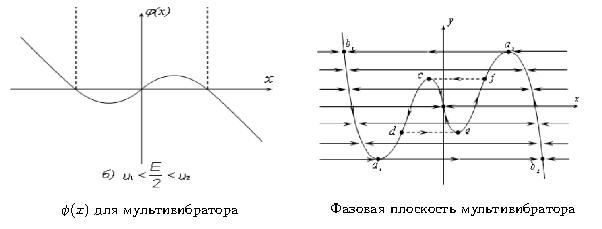
\includegraphics[width=1\textwidth]{plot/ris1}
       \vspace{-1.4em}
     \caption{}
     \label{fig:dummy}
	\end{figure}
Нами были измерены период автоколебаний мультивибратора $T$ и их амплитуда $A$: 
\begin{equation}
	T=68 \text{ мкс}, \quad A = 0.8 \text{ В}
\end{equation}
   \begin{figure}[H]
    \centering
       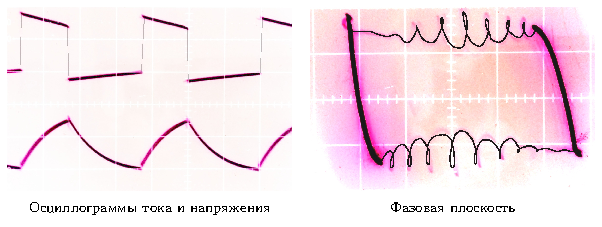
\includegraphics[width=1\textwidth]{plot/multi}
       \vspace{-1.4em}
     \caption{}
     \label{fig:dummy}
	\end{figure}
На фазовой плоскости и осциллограмме напряжения (сверху) хорошо видны быстрые (скачкообразные) и медленные движения системы. А фазовая плоскость позволяет увидеть существование устойчивого предельного цикла.

% \newpage
\subsection{Режим триггера}
\begin{figure}[H]
	\centering
	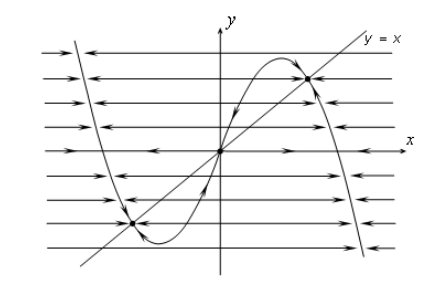
\includegraphics[width=0.5\textwidth]{photo/trigger}
	\caption{Фазовая плоскость триггера}
	\label{fig:tr}
\end{figure}
Триггер (его так же называют бистабильным мультивибратором) -- система, имеющая два устойчивых и одно неустойчивое состояния равновесия, которая может быть переброшена из одного состояние в другое подачей соответствующего импульса система в подходящий узел схемы. 
$\varphi(x)$ для триггера такое же, как и для мультивибратора, однако $\varphi'(0)>1$ (см. рис. \ref{fig:tr}).

Мы сняли длительность снимаемого импульса на определенной частоте: $52$ мкс на частоте $7.2$ кГц.

\subsubsection{Влияние длительности запускающего импульса на переброс триггера}
   \begin{figure}[H]
    \centering
       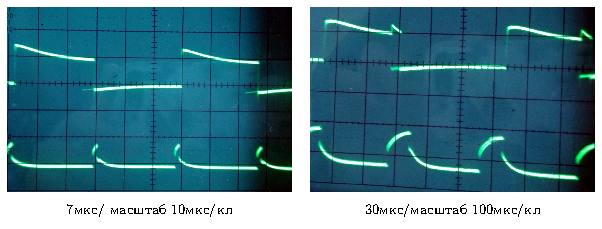
\includegraphics[width=1\textwidth]{plot/ris2}
       \vspace{-1.4em}
     \caption{Влияние длительности запускающего импульса на переброс триггера}
     \label{fig:dummy}
	\end{figure}

Существует пороговое значение длительности запускающего импульса, ниже которого движение по траекториям медленных движений не происходит. При длительности 30 мкс уже появляются видимые искажения, то есть из-за плавного роста амплитуды запускающего импульса не сразу получается перебросить систему в другое состояние.

Таким образом, минимальное значение длительности запускающего импульса: $T_{min} = 7$ мкс.
Максимальное (при котором появляются заметные искажения): $T_{max} = 30$. При $T = 80$ мкс искажения уже очень велики. 

\subsubsection{Влияние амплитуды запускающего импульса на переброс триггера}
Существует пороговое значение амплитуды, ниже которого режим триггера не работает ($U = 0.75$ В, $\tau = 20$ мкс, $f = 7.2$ кГц). Дальнейшее увеличение амплитуды никак не влияет на переброс триггера.

\subsubsection{Деление частоты на триггере}
Деление частоты на триггере - режим триггера, при котором период следования импульсов меньше времени разрешения триггера в $n$ раз, где $n$ - целое число. В работе исследуется деление частоты на триггере при $n = 2$.
  
\begin{figure}[H]
	\centering
	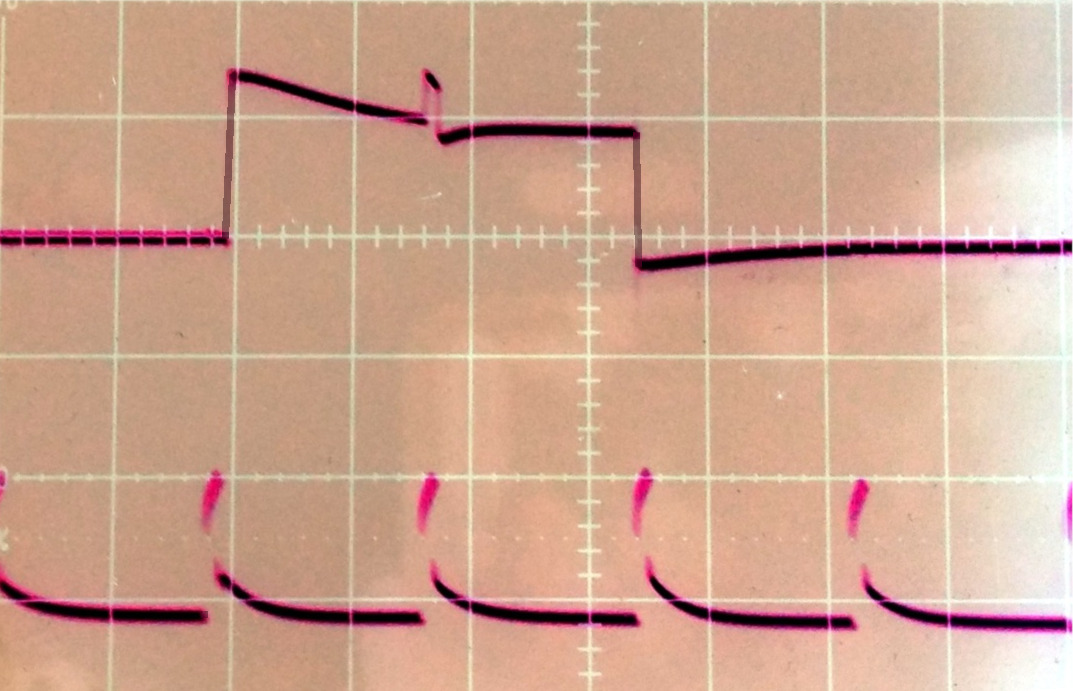
\includegraphics[width=0.5\textwidth]{photo/del_f}
	\caption{Деление частоты на триггере, $f = 5$ кГц}
	\label{fig:figure2}
\end{figure}

Отсутствие реакции системы в нижнем состоянии на второй импульс может быть обусловлено несимметричностью схемы установки. Однако точно видно, что \textbf{для переброса системы из одного состояния в другое необходимо два импульса}. Деление частоты на триггере было получено при $f = 5$ кГц. 

Следовательно, время разрешения триггера $T$: 
\begin{equation}
	T = 2 \cdot \frac{1}{f} = 0.4 \cdot 10^{-3} \text{ с}
\end{equation}

\subsection{Режим кипп-реле}
\begin{figure}[H]
	\centering
	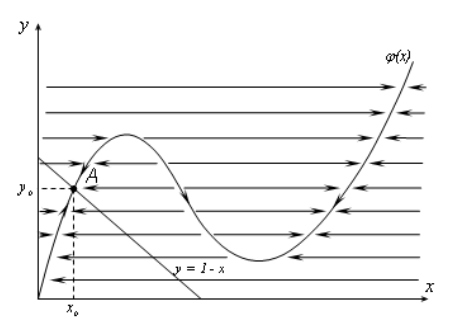
\includegraphics[width=0.7\textwidth]{photo/kipp}
	\caption{Фазовая плоскость кипп-реле}
	\label{fig:figure2}
\end{figure}

Кипп-реле (одновибратор) -- система, которая на одиночный импульс реагирует также одиночным импульсом, но другой длительности и с задержкой. Причем выходной сигнал зависит только от параметров системы.

Длительность входного импульса: $1.5$ мкс. Длительность выходного сигнала: $3$ мкс.

Схема работает как кипп-реле при длительности входного импульса: 
$$0.15 \text{ мкс}<\tau<1.8 \text{ мкс}$$

Существуют также пороговые значения амплитуды. Так, на частоте $f = 7$ кГц и длительности входного импульса $\tau = 1.5$ мкс, система работает как кипп-реле при амплитуде входного импульса: $0.06 \text{ В}<U<2\text{ В}$
\end{document}